

\section{Map Projections}
Our search for a simpler model which depicts the Earth's surface which could represent the whole globe has lead us to map projections.
There are numerous map projections, which are being used to represent for different areas of the Earth. An preliminary overview to the map projections is needed and how map projections are generated and how Earth's models explained in the previous section are related to map projections.

A map projection is a way to represent some part or the whole surface of the Earth on a two dimensional plane, this procedure of mapping the three dimensional surface to a plane is done using mathematical calculations.
Map projections brings us a to represent the whole Earth but each and every map projection is subjected to distortions in shape, area, angles and distance. If one of the map projection try to minimize or mitigate one or two of the distortions, that projection would still be subjected to a distortion.

\subsection{Generation of Map Projections}
The creation of the map projections require us the usage of \textbf{developable surfaces}. The characteristic which is required for creating the map projections is that they can be mapped onto a two dimensional plane isometrically\cite{Patrikalakis_Maekawa_2010}.
There are three major types of developable surfaces, cylinder, cone, and plane which are used for generating map projections.

The general procedure for generating a map projection is that we first select a geoid model and a reference ellipsoid for approximating the underlying geoid. After the approximation using the geoid then a developable surface is selected from the above mentioned developable surfaces.
Then wrapping the globe with the developable surface gives us the desired map projection.

\begin{figure}[H]
    \centering
    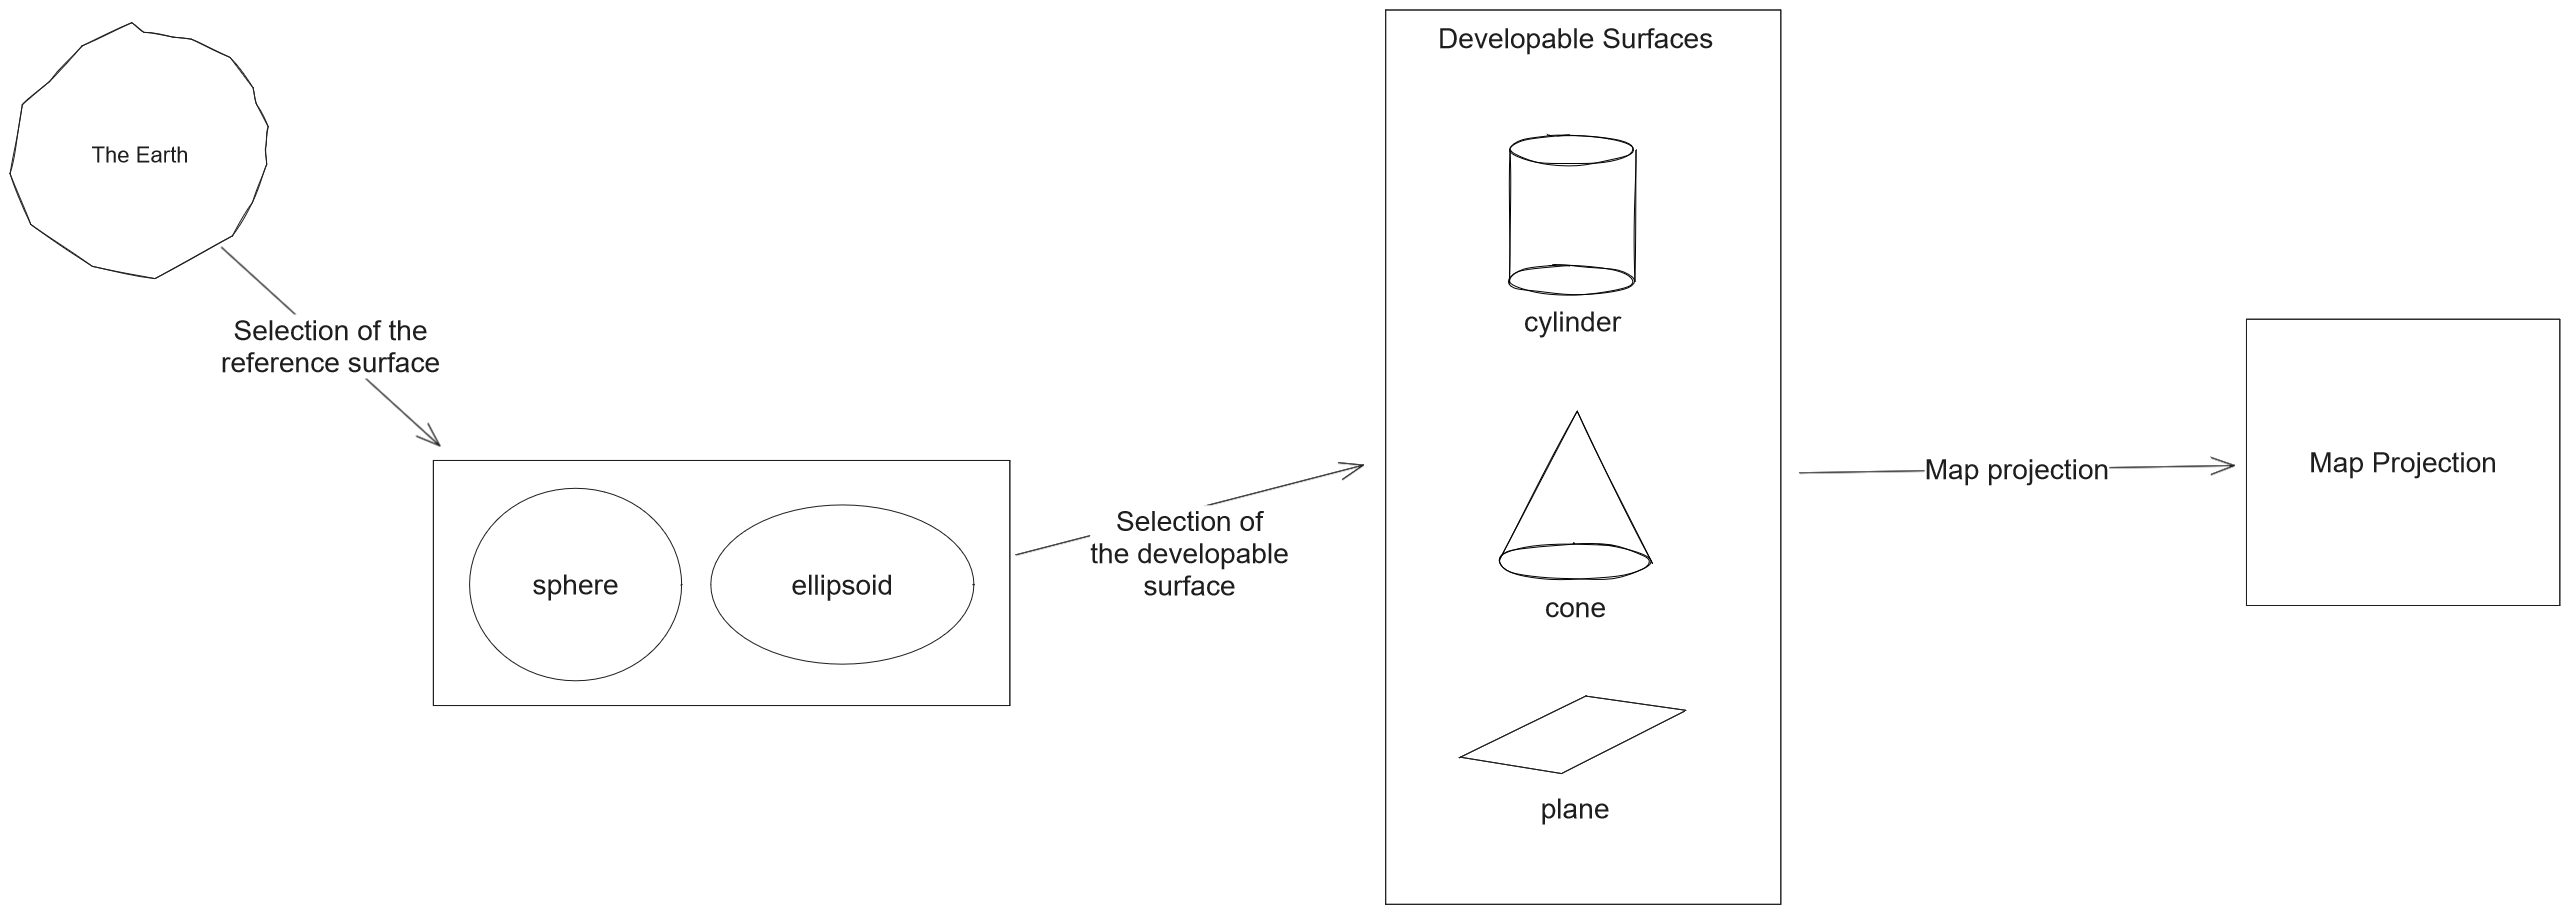
\includegraphics[width=1.0\textwidth]{figures/chapter-3/map_projection_creation.png}
    \caption{Map projection generation flowchart  }
    \label{fig:earth-image}
\end{figure}

\subsection{Types of Map Projections}

The map projections are classified on the bases of the developable surface used for their creation. There are three major types of map projections

\begin{itemize}
    \item Cylindrical Projections
    \item PseudoCylindrical Projections
    \item Conic Projections
    \item Planar (Azimuthal) Projections
\end{itemize}

\subsubsection{Cylindrical Projections}
\begin{figure}[h]
    \centering
    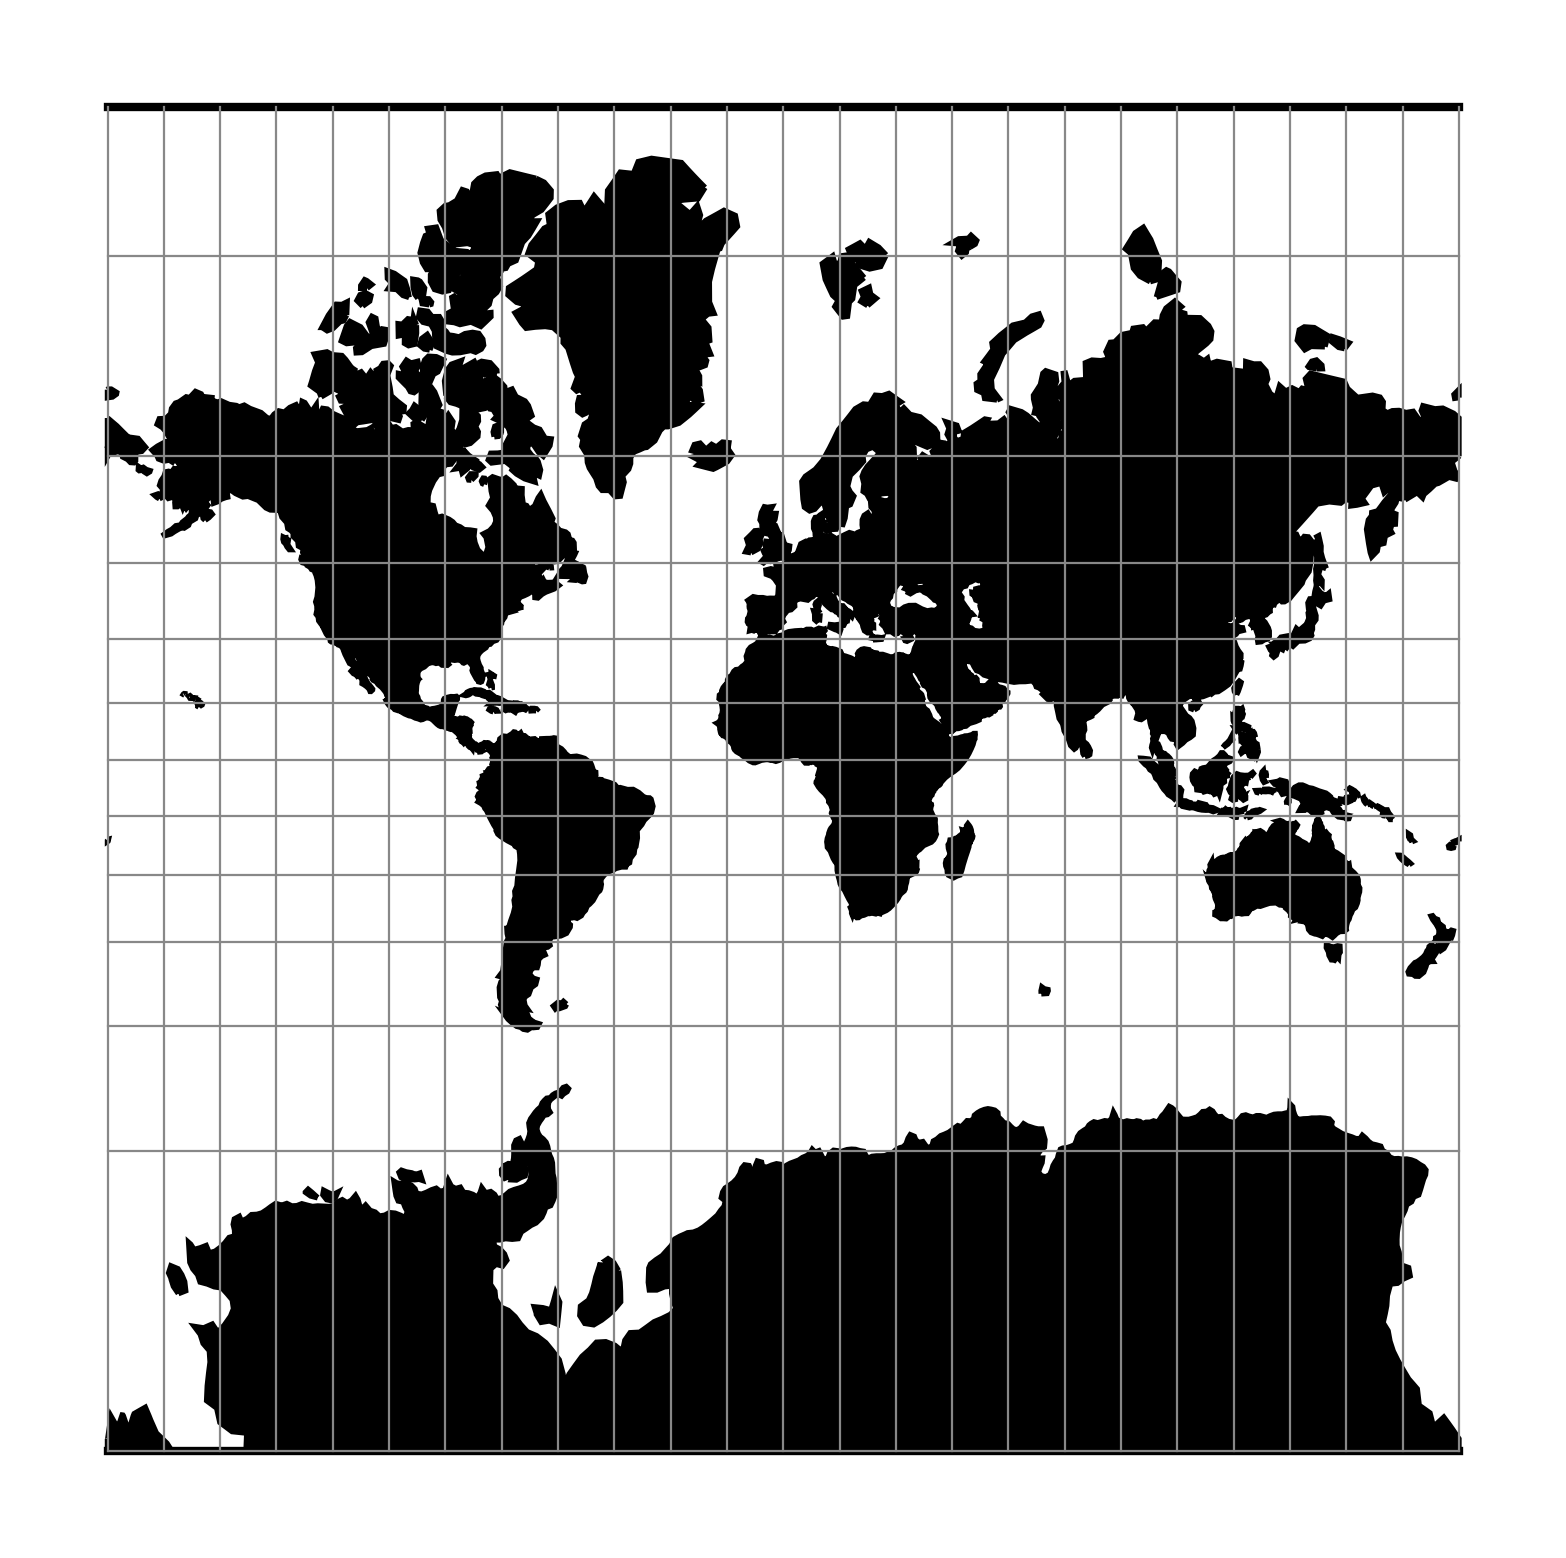
\includegraphics[width=0.5\textwidth]{figures/chapter-3/merc.png}
    \caption{Mercator Map Projection (Source \cite{PROJ_SITE})}
    \label{fig:merc}
\end{figure}

Cylindrical map projections are generated when the Earth is enveloped by a cylinder, same as we place the globe at the center. All of the longitudinal lines will be projected on the cylinder as perpendicular lines to the equator and the latitudinal lines  will be parallel to the equator. If we cut the cylinder at any of the longitude we have a cylindrical projection \cite{Snyder1982}.

In the image above Mercator projection is shown, which has conformal property (preserves the shape and the angles), but the size of the land mass is distorted at the polar regions \cite{GISGEO_Cylinder}. Where Greenland is bigger than African continent, in reality that is not true.


\subsubsection{Pseudocylindrical Projections}

\begin{figure}[h]
    \centering
    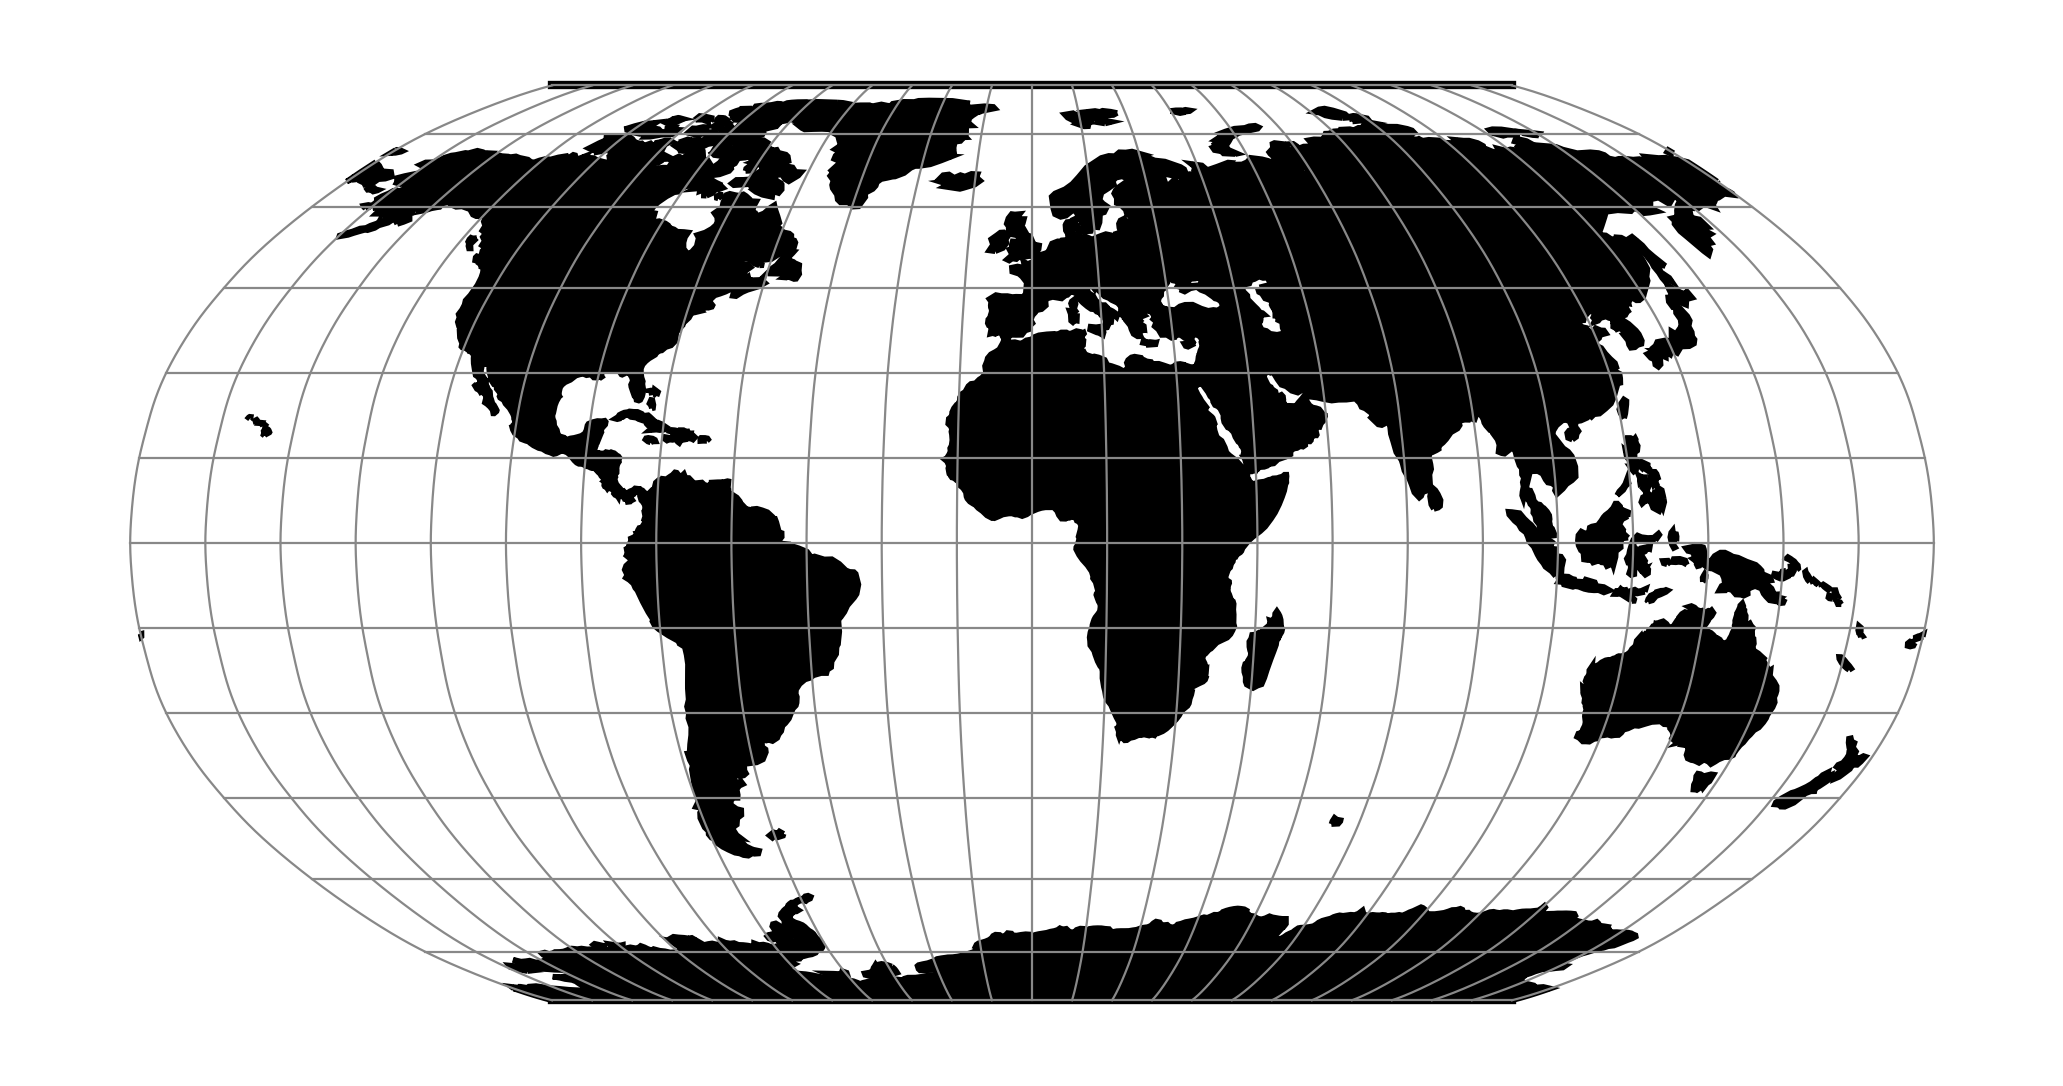
\includegraphics[width=0.5\textwidth]{figures/chapter-1/robinson.png}
    \caption{Robinson Map Projection (Source \cite{PROJ_SITE})}
    \label{fig:robinson-image}
\end{figure}


These projections are generated using the same method as cylindrical projections are created but the longitudinal lines are curved other than the prime meridian but the latitudinal lines are parallel to the equator \cite{GISGEO_Cylinder}.
The above image shown is the robinson projection which is a pseudocylindrical projection.

\subsubsection{Conic Projections}

\begin{figure}[h]
    \centering
    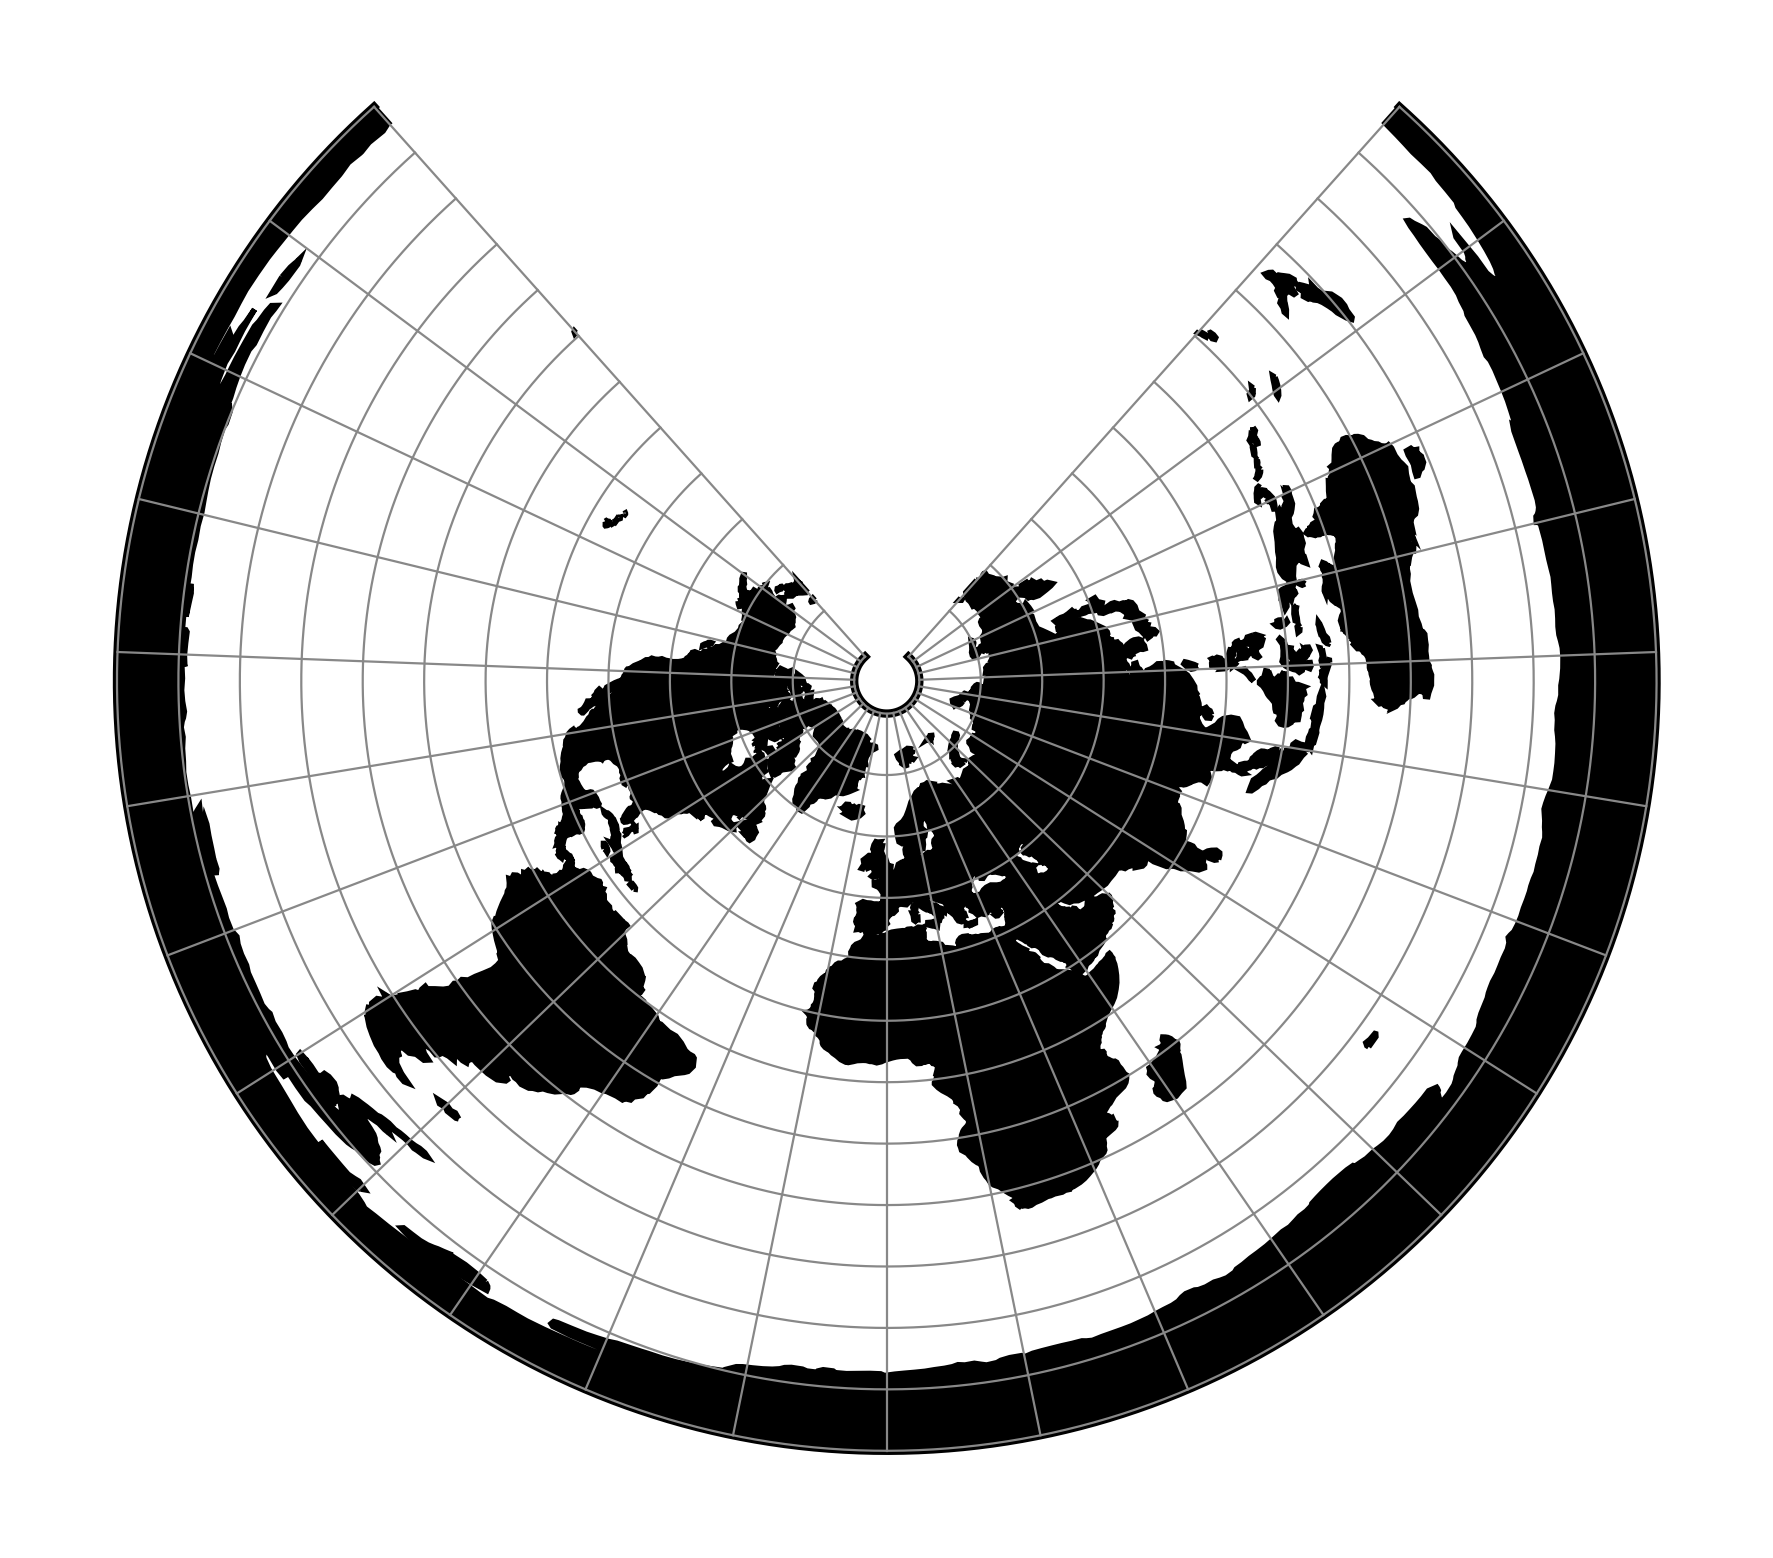
\includegraphics[width=0.5\textwidth]{figures/chapter-3/vitk1.png}
    \caption{Vitkovsky I Map Projection (Source \cite{PROJ_SITE})}
    \label{fig:vitkovsky-image}
\end{figure}
Conic projections are formed by situating a cone atop the Earth's pole and completely enveloping the Earth within the cone. Consequently, the longitudinal lines remain linear, while the latitudinal lines become arcs that revolve around the apex of the cone. Upon severing the cone along any given longitudinal line, a conic projection is thereby produced \cite{Snyder1982}.

\subsubsection{Planar Projections}

\begin{figure}[h]
    \centering
    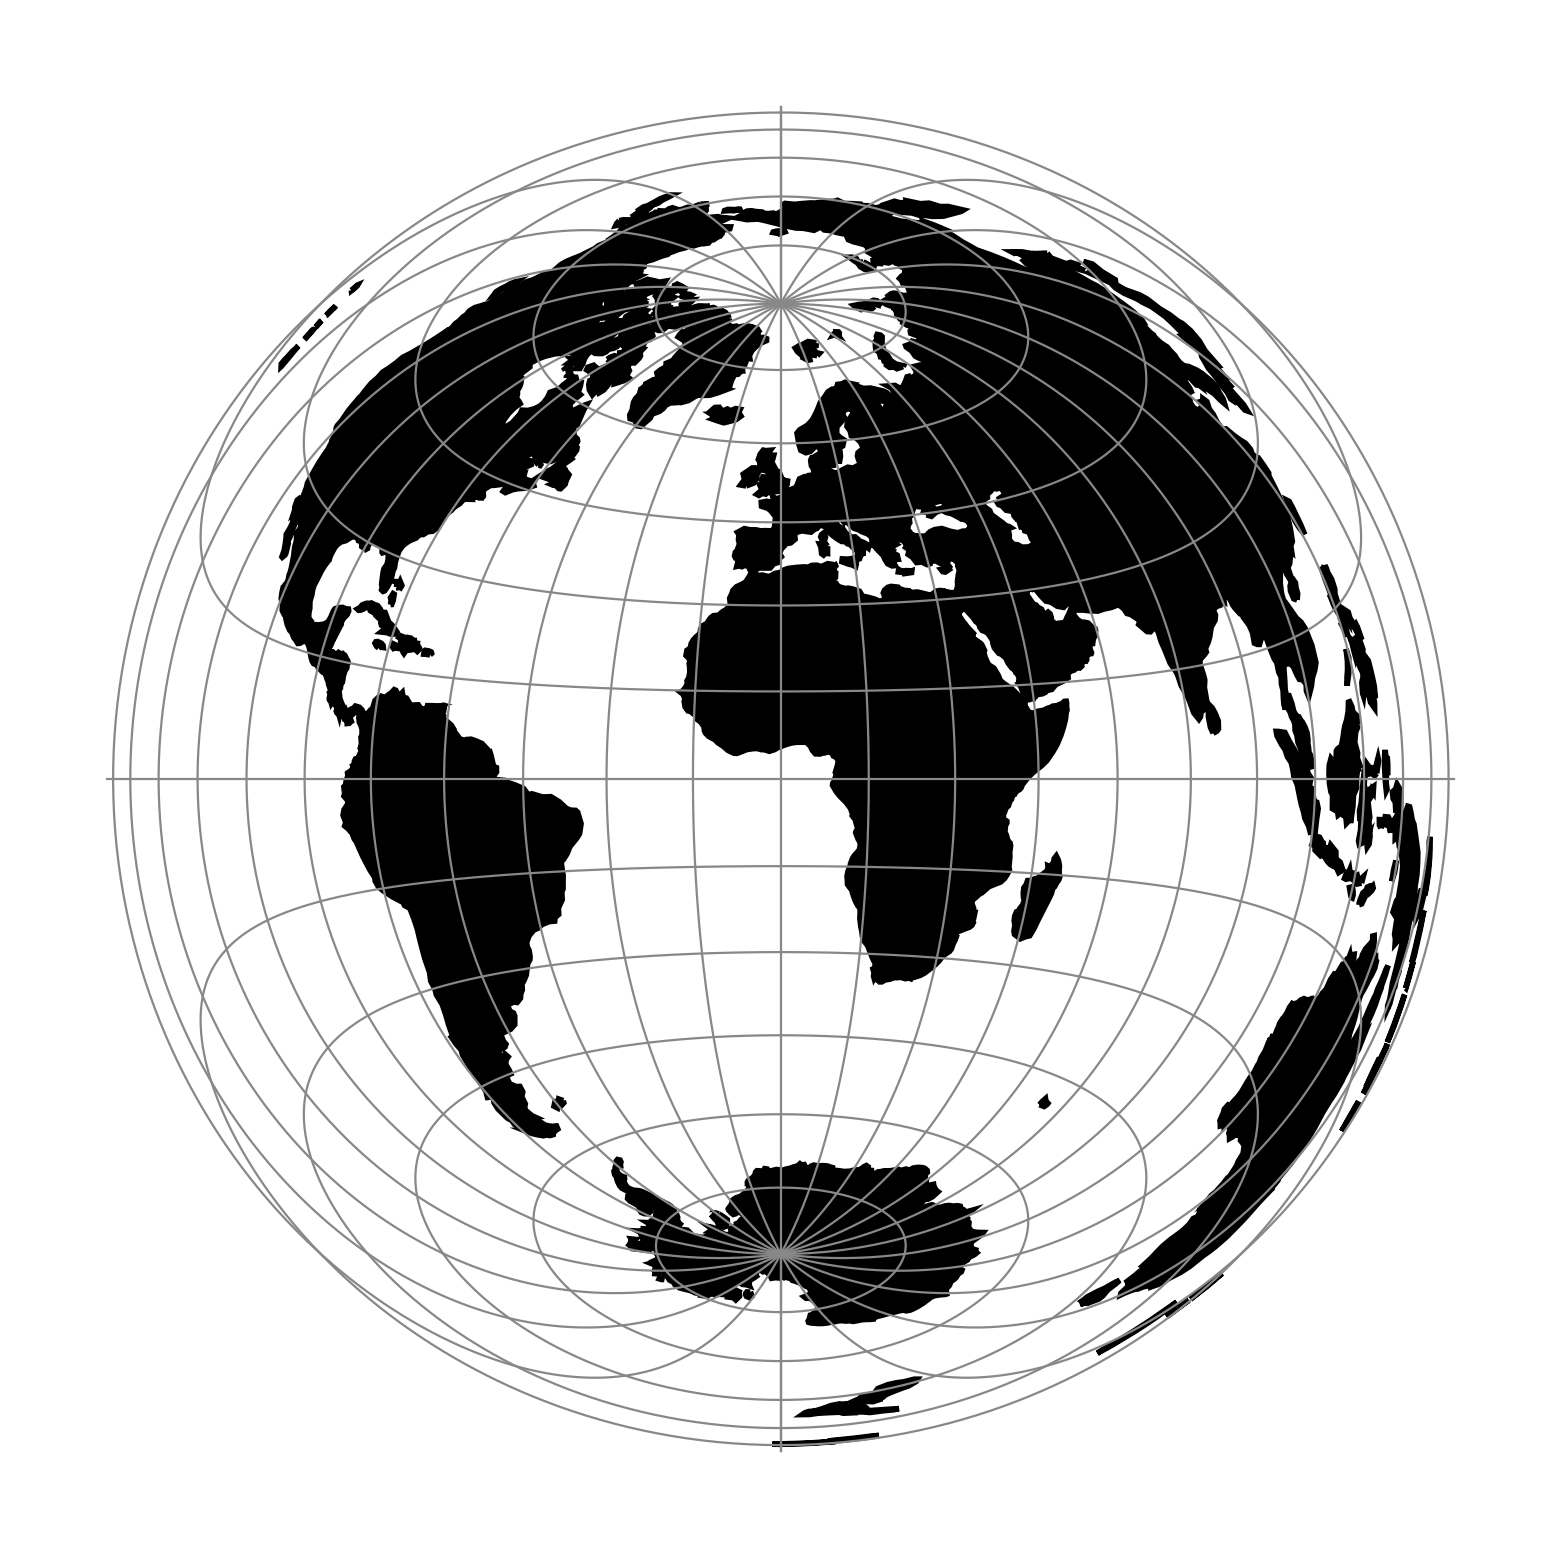
\includegraphics[width=0.5\textwidth]{figures/chapter-3/laea.png}
    \caption{Lambert Azimuthal Equal Area Map Projection (Source \cite{PROJ_SITE})}
    \label{fig:vitkovsky-image}
\end{figure}

planar projections are formed when the plane is positioned at one of the Earth's poles and is tangent to the sphere. Consequently, the projection of the sphere becomes azimuthal. In this scenario, the longitudinal lines will appear as straight lines originating from the point of tangency \cite{Snyder1982}.


\subsection{Map Projections and Distortions}
\begin{figure}[H]
    \centering
    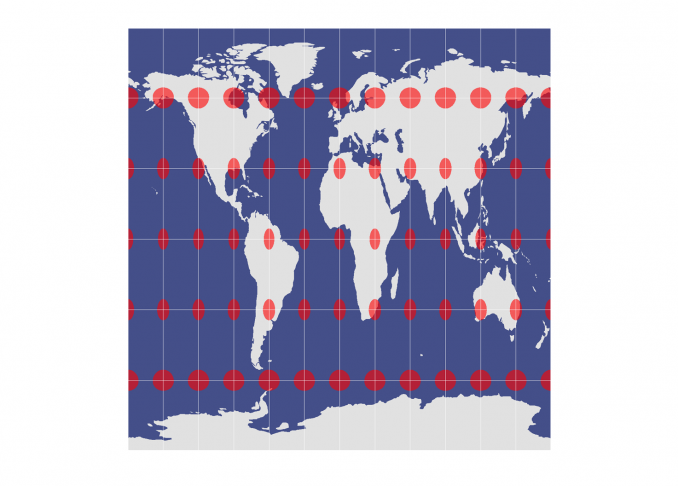
\includegraphics[width=0.5\textwidth]{figures/chapter-3/Tissot-Equidistant-Cylindrical-1-678x486.png}
    \caption{Tissot's Indicatrix on Equidistant Cylindrical Projection (Source \cite{GISGEO_Tissot})}
    \label{fig:tissot-image}
\end{figure}
Whenever a three dimensional geometric shape is projected to a two dimensional geometric shape, there will be distortions. same is the case with the map projections which are projection of our three dimensional Earth to two dimensional plane.
The distortions in map projections can be categorized into four types:
\begin{itemize}
    \item Area distortion
    \item Direction distortion
    \item Shape distortion
    \item Distance distortion
\end{itemize}

To gain a better understanding of these distortions, Tissot's indicatrix can be utilized, it visually demonstrates the distortions by depicting ellipses, known as indicatrices, which change their shape to represent the distortions \cite{Snyder1982}.
\begin{itemize}
    \item The preservation of local angles and shapes is ensured through the utilization of conformal map projections \cite{GISGEO_Tissot}.
    \item The preservation of the relative size of areas is achieved through the utilization of Equal Area Projections \cite{GISGEO_Tissot}.
    \item The distance on certain set of lines is preserved by Equidistant Projections \cite{GISGEO_Tissot}.
\end{itemize}
Figure ~\ref{fig:tissot-image} shows the tissot's indicatrix on the Equidistant Cylindrical projection which tries to preserve distances along the equator and the longitudinal lines only \cite{GISGEO_Tissot}.